\section{Обоснование структуры системы в защищённом исполнении} \label{model}

В рамках разработки защищенной системы электронного документооборота необходимо обеспечить решение следующих задач:
\begin{itemize}
	\item предоставление пользователю интерфейса использования функций разрабатываемого ПО;
	\item управление учётными записями пользоваетлей;
	\item идентификация и аутентификация пользователей;
	\item передача документов и метаданных;
	\item обработка вносимых в документ и метаданные изменений;
	\item хранение внесённых изменений;
	\item отображение истории внесённых изменений и текущего состояния документа.
\end{itemize}

\vspace{\baselineskip}
В качестве основных требований к конструкции ПО можно указать следующие:
\begin{itemize}
	\item конструкция ПО не должна отрицательно влиять на производительность;
	\item пользователь ПО должен быть обеспечен удобным интерфейсом для работы;
	\item конструкция разрабатываемого ПО должна способствовать обеспечению достаточного уровня производительности;
	\item конструкция разрабатываемого ПО должна соответствовать выбранной в исследовательской части.
\end{itemize}

\vspace{\baselineskip}
Рассмотренные задачи и требования обуславливают следующую структуру системы (рис. \ref{img:modules})
\begin{figure}[h!]
  \centering
  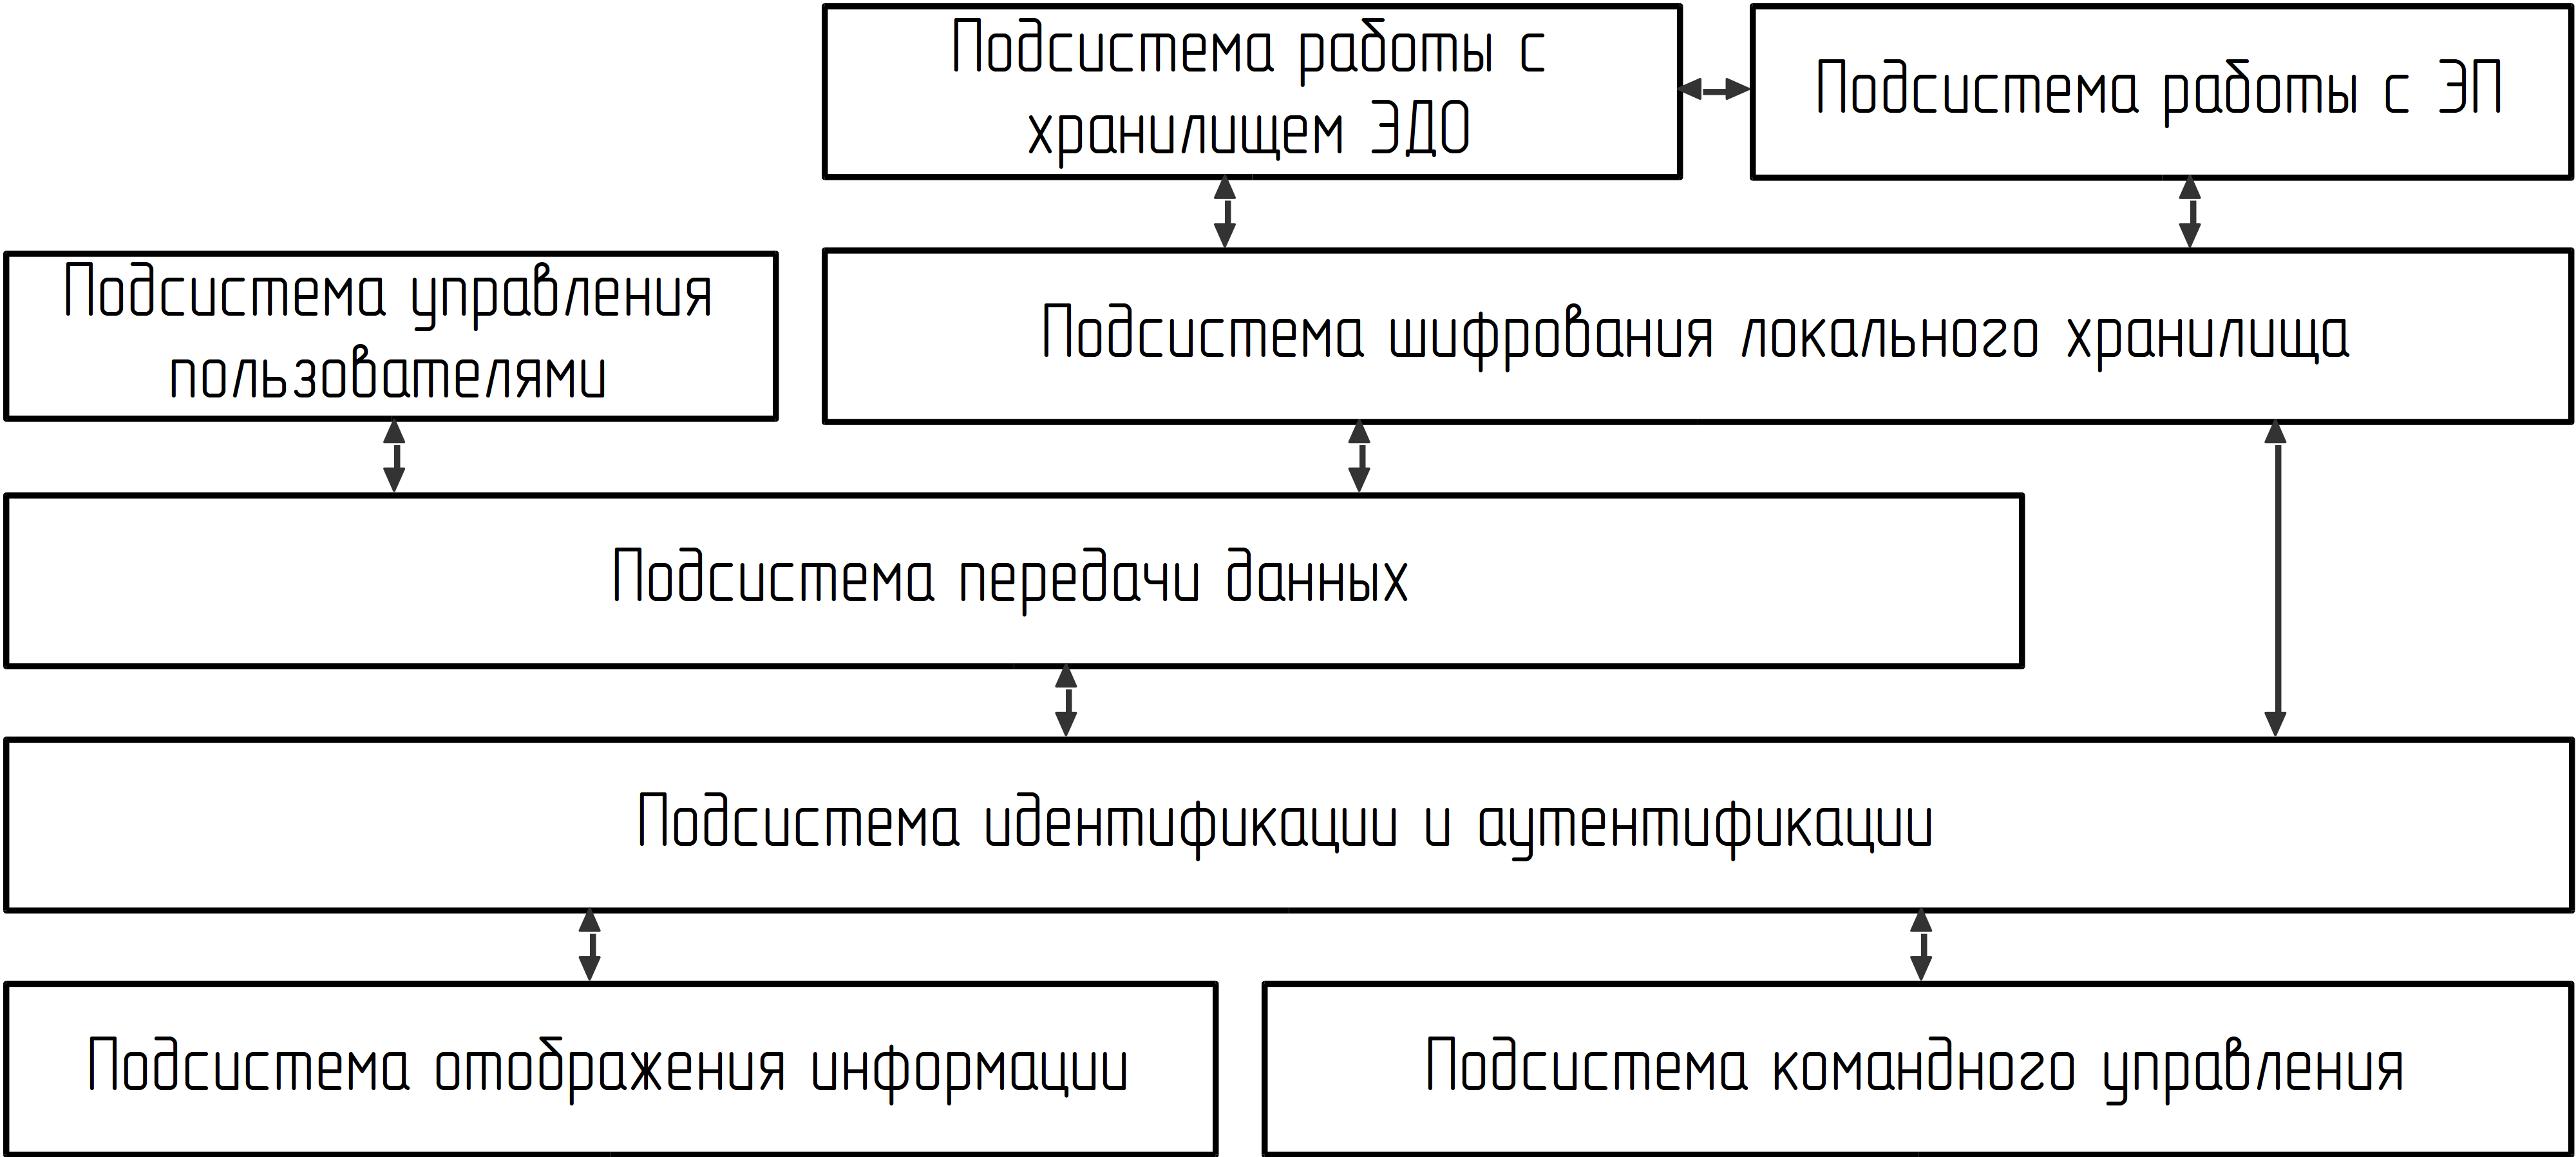
\includegraphics[width=1\textwidth]{modules}
  \caption{Общая структура разрабатываемого ПО}
  \label{img:modules}
\end{figure}

\vspace{\baselineskip}
\textbf{Подсистема графического интерфейса} должна обеспечивать:
\begin{itemize}
	\item возможность просмотра истории документов;
	\item возможность просмотра сотояния любого документа в любой момент времени;
	\item возможность проверки статуса электронной подписи записей истории.
\end{itemize}

\vspace{\baselineskip}
\textbf{Подсистема командного управления} должна обеспечивать предоставления интерфейса для выполнения всех функций системы.

\vspace{\baselineskip}
\textbf{Подсистема идентификации и аутентификации} выполняет проверку идентификаторов пользователей и осуществляет их аутентификацию в системе.

\vspace{\baselineskip}
\textbf{Подсистема передачи данных} отвечает за передачу данных между клиентами и серверами по защищённому каналу в случае необходимости. Защита канала осуществляется по протоколам ssh и https.

\vspace{\baselineskip}
\textbf{Подсистема управления пользователями} реализует механизм разграничения доступа.

\vspace{\baselineskip}
\textbf{Подсистема шифрования локального хранилища} обеспечивает шифрование ХЭД как на стороне клиента, так и на стороне сервера. Может быть ореализована на основе TrueCrypt или другой подобной системы.

\vspace{\baselineskip}
\textbf{Подсистема работы с электронной подписью} реализует операции создания и проверки электронной подписи. Использует механизмы GPG и OpenSSL.

\vspace{\baselineskip}
\textbf{Подсистема работы с хранилищем электронных документов} реализует все функции работы с документами и их историей, кроме тех, которые требуют проведения криптографических операций.

\vspace{\baselineskip}
Общий алгоритм действий программы представлен на рис. \ref{img:algorithm-horizont}.

\vspace{\baselineskip}
Как следует из представленной структуры, разрабатываемое ПО имеет сложную многокомпонентную структуру, что обуславливает целесообразность реализации программных средств не как автономно работающего приложения, а как программного пакета, содержащего исполняемые модули, библиотеки данных и другие информационные ресурсы.

\vspace{\baselineskip}
К достоинствам такого подхода можно отнести масштабируемость, простоту разработки, а также возможность более гибкого распределения задач между программистами при организации управления программным проектом.

\begin{landscape}
\begin{figure}[h!]
  \centering
  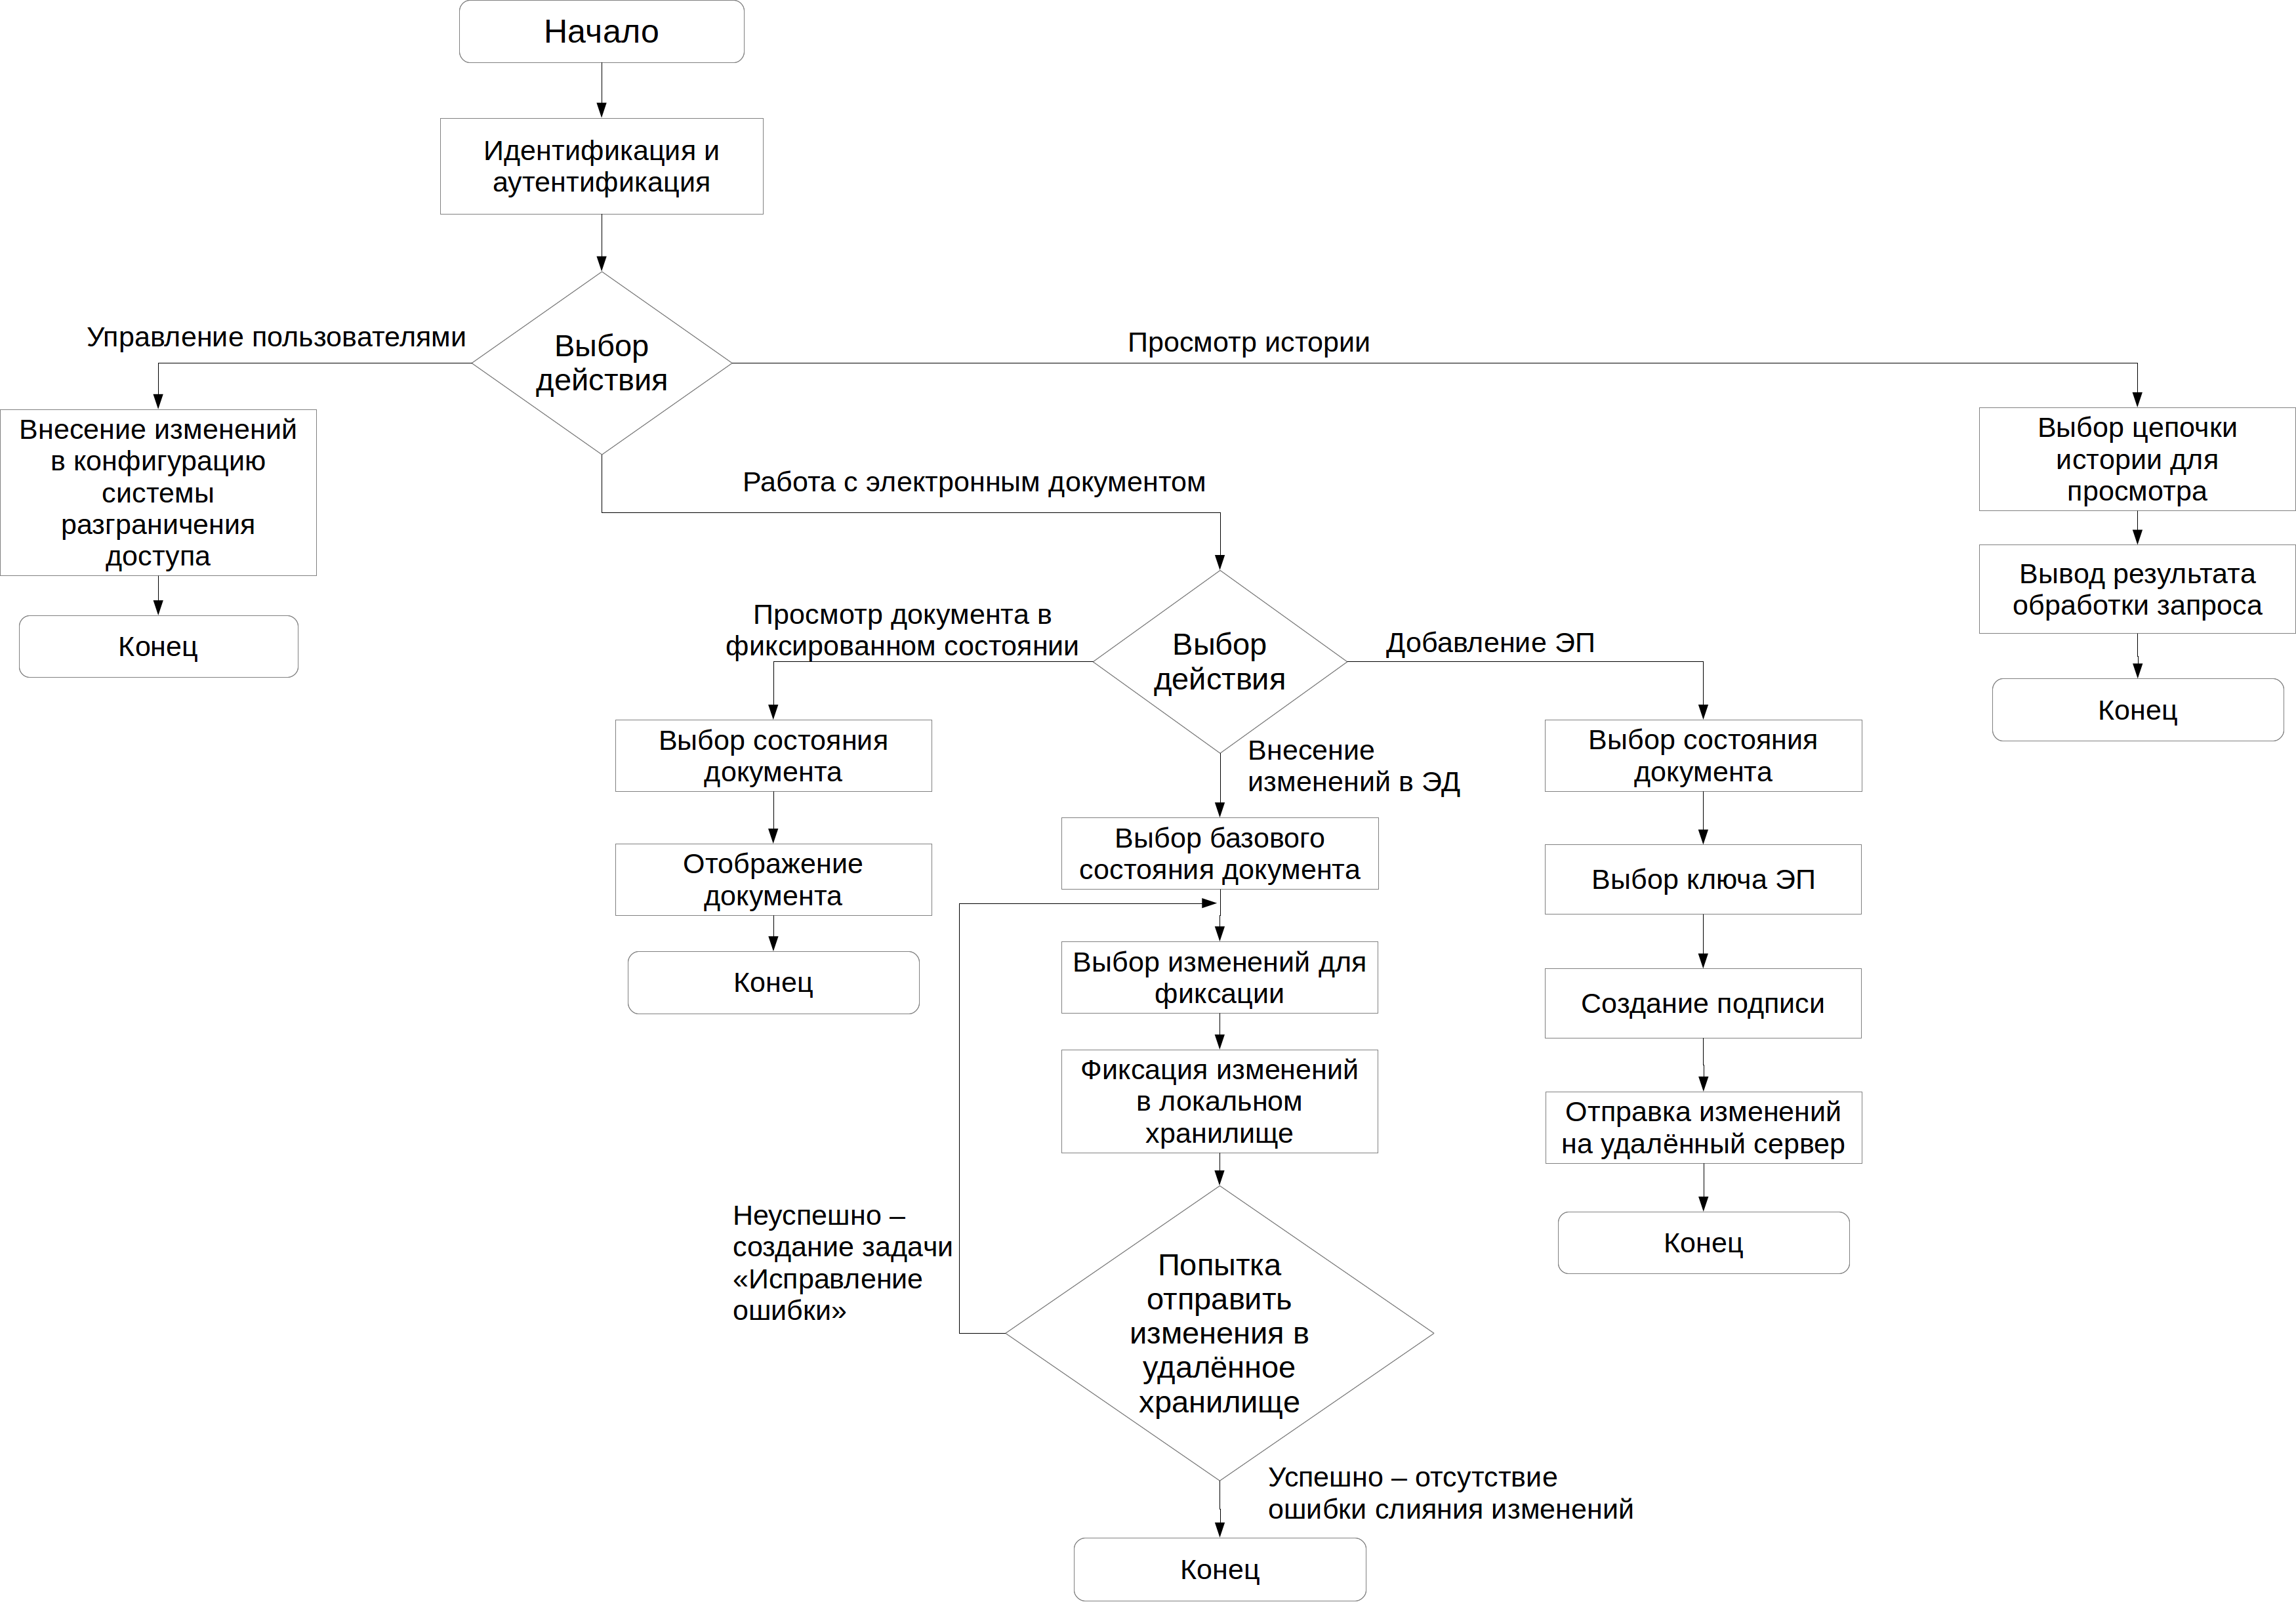
\includegraphics[width=1.35\textwidth]{algorithm-horizont}
  \caption{Общий алгоритм действий программы}
  \label{img:algorithm-horizont}
\end{figure}
\end{landscape}